\section{Unit testing}
Unit test procedures were conducted after the development of each module, reviewed and verified for correspondence to component level design. The data extraction module was tested to ensure that only the required data is collected. We also made sure that the data we collected are in our expected format. . All of the unit test cases covered the interface to the module to ensure proper flow of data, the local data structures used to ensure integrity of data during execution and boundary conditions. Input combinations were chosen to exercise all independent paths and error handling paths. The following were the unit test cases designed and implemented:
\subsection{Web Interfaces}
\subsubsection{Search Module}
Test cases were designed to ensure that all relationships are displayed. Tests made sure that when the fields are empty and when no relationship exists for a node appropriate “search unsuccessful” messages are shown. Tests were conducted to ensure that failure messages are display upon any failures due to error in connection to databases.
\subsubsection{Process Node module}
Test cases were designed to ensure that nodes are properly added and deleted from the database It was ensured that the Node Table and graph database was updated whenever a node was added or deleted .Tests were also conducted to ensure that unsuccessful and failure messages are shown accordingly.
\subsubsection{Process Relationship module}
Test cases were designed to ensure that relationships were inserted deleted and updated correctly. It was also ensured that empty fields displayed error messages. Failure and unsuccessful message paths were also exercised.

\section{Integration Testing}
Integration testing is a systematic technique for constructing the program structure while conducting tests to uncover errors associated with interfacing. The objective is to take the unit tested modules and build a program structure that has been dictated by design.
Incremental integration testing was followed. The strategy used was bottom up integration. It was implemented in the following way:
\begin{itemize}
\item The data extraction module and the NLP module were integrated to form a cluster. The data correctly extracted was stored in the PostgreSQL database.
\item Output from the cluster was fed into the middleware module, in which the taxonomy classification was performed.
\item Next part of testing was integrating the output of the middleware module with the Graph database. The graph was displayed in the web interface.
\end{itemize}
Each time a new module was added, regression testing was performed. This involved re-testing the previously tested modules by re-execution of some of the subsets of tests that had already been performed to ensure that the addition of new modules has not led to unintended side effects. 

\section{Validation testing}
\par
A series of black box tests were conducted to ensure that all functional requirements were satisfied, all behavioral characteristics were achieved and all performance requirements were attained. Conformity to reasonable expectations outlined in the Software Requirements Specifications under validation criteria was checked with.It was ensured that all the web pages were directed correctly from one page to another in case of the web interface provided. 
\paragraph*{Alpha and beta testing}The alpha version of the application was tested by the teachers and the other students who were not part of this team. The beta version of the application has not yet been launched.

\section{System Testing}
System testing is actually a series of different tests whose primary purpose is to fully exercise the computer based system. The following types of systems tests were performed.
\section{Recovery Testing}
Recovery testing is a system test that forces the system to fail in a variety of ways and verifies that recovery is properly performed. In this case the system was forced to fail in variety of ways for example by disconnecting PostgreSQL while still retaining connections to graph database. It was ensured that in all such situations the system is consistent.
\section{Performance Testing}
For real time systems, software that provides the required functions but does not conform to performance requirements is unacceptable. Thus run-time performance test of software within the context of an integrated system is very important. Performance testing was done at all stages of the development of this project. Performance of each individual module was tested individually and it was verified that each module conforms to the requirements. After this all the modules were integrated and tested. The database was expanded sufficiently to verify that the performance does not degrade with increase in data.
\section{Results}
\subsection{Final Application}
\subsubsection{Web Interface}
\begin{figure}[h]
	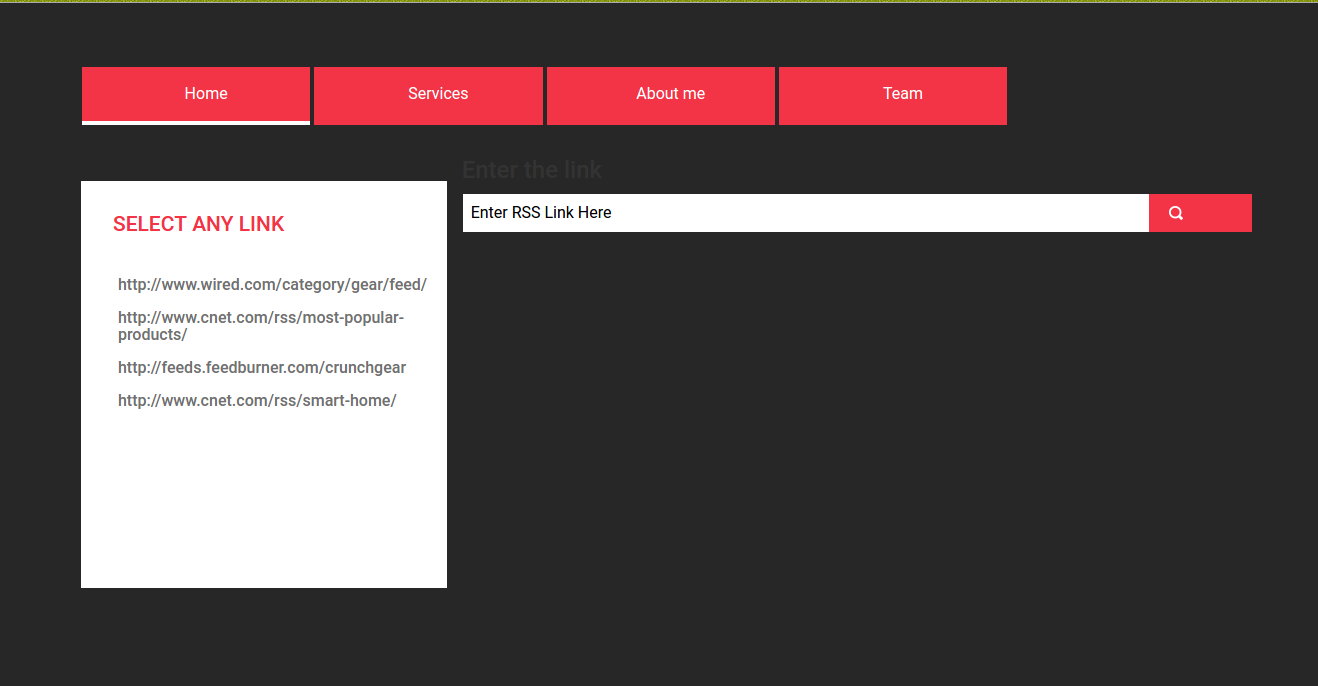
\includegraphics[width=13cm, height=8cm]{naiveUser}
	\centering
	\caption{Interface provided for the naïve user}
	\label{fig:naiveUser}
\end{figure}
Interface provided for the naïve user is shown in figure \ref{fig:naiveUser}. User can enter the link of the RSS feed he need to inspect, or he can select any of the links we have provided.

\begin{figure}[h]
	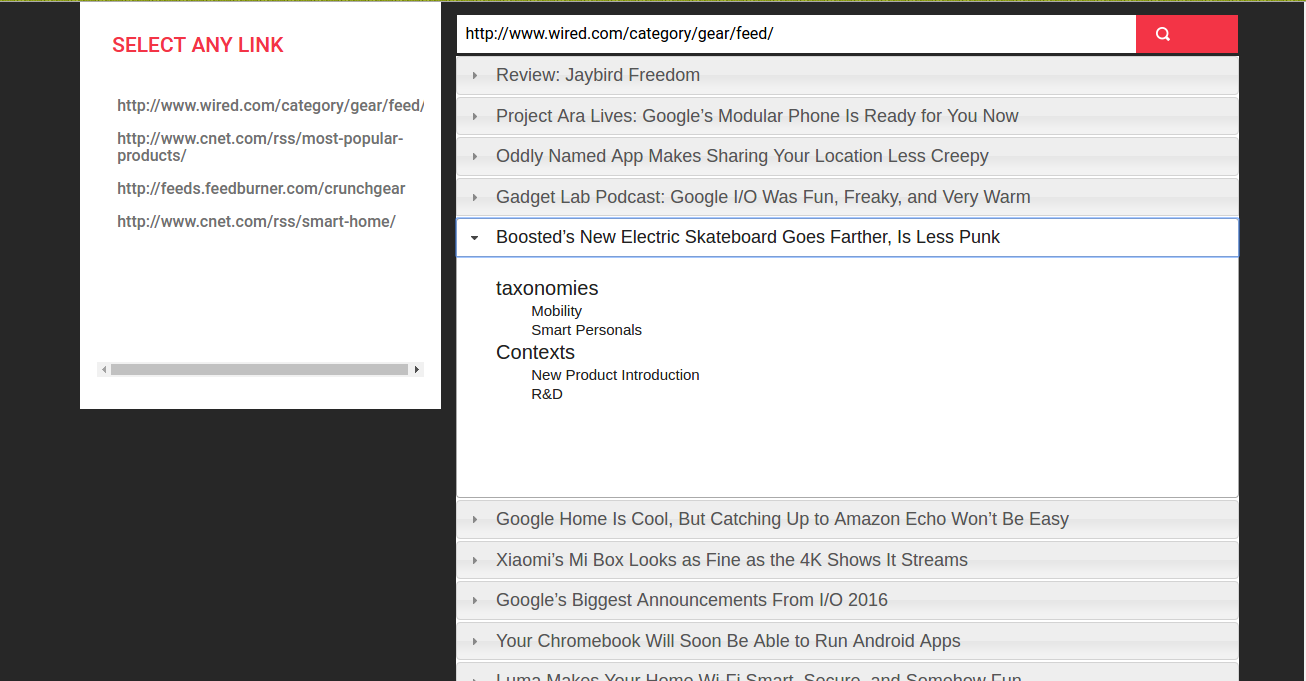
\includegraphics[width=13cm, height=8cm]{naiveUserContent}
	\centering
	\caption{Screenshot of the page when content of a link is extracted}
	\label{fig:naiveUserContent}
\end{figure}
The figure \ref{fig:naiveUserContent} shows the screenshot when the content of a link is extracted.

\begin{figure}[h]
	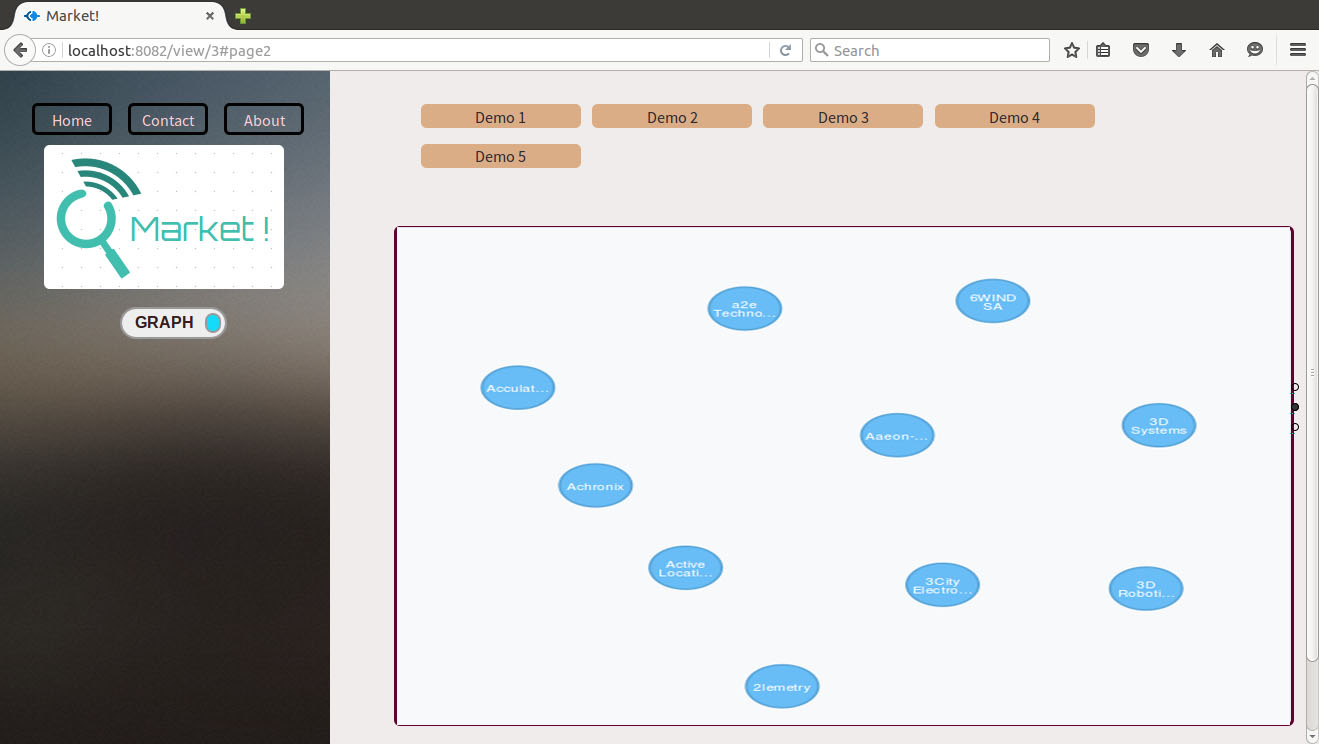
\includegraphics[width=13cm, height=8cm]{queryDatabase}
	\centering
	\caption{Screenshot of the page when user to query the graph database}
	\label{fig:queryDatabase}
\end{figure}
The figure \ref{fig:queryDatabase} shows screenshot of the interface used by the user to query the graph database and see the results.
\paragraph*{D3 Visualizations}
\begin{figure}[h]
	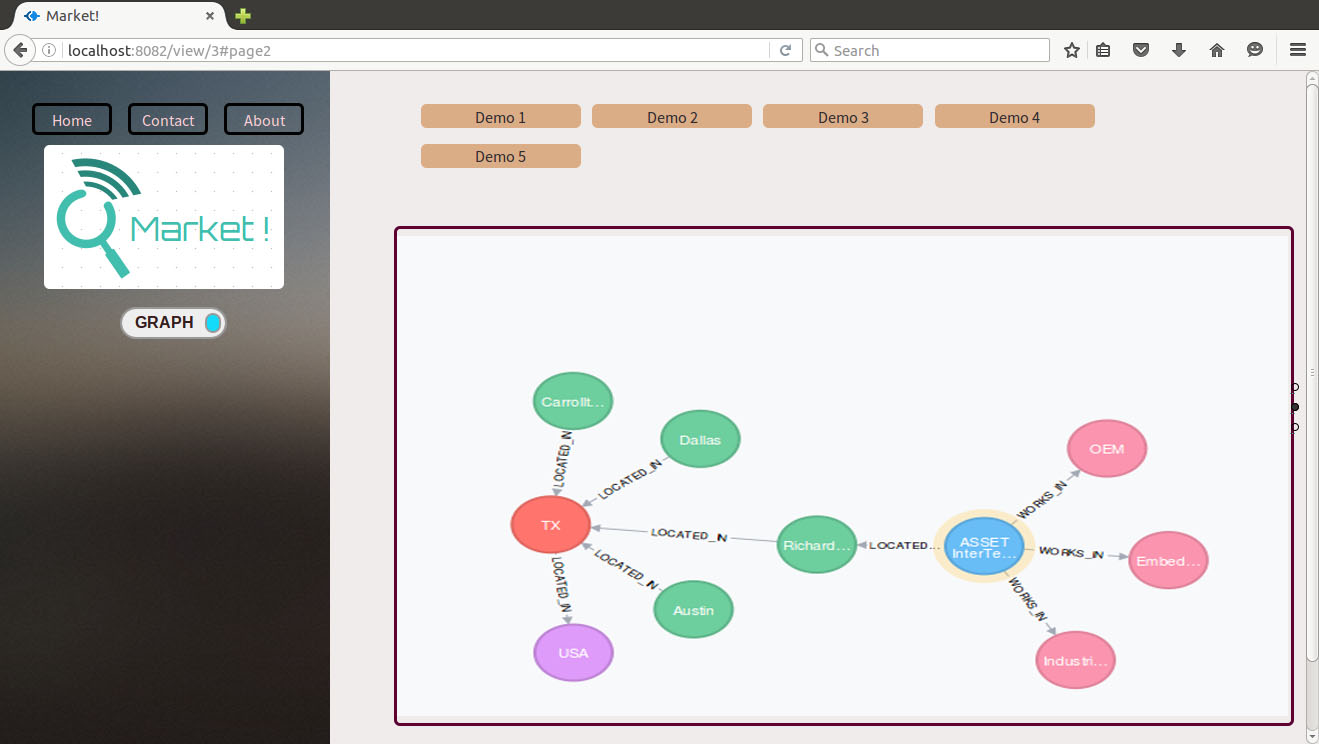
\includegraphics[width=13cm, height=8cm]{d3visual1}
	\centering
	\caption{Example Query: Querying of Asset Technologies}
	\label{fig:d3visual1}
\end{figure}
Figure \ref{fig:d3visual1} shows the screenshot which displays the query of Asset Technologies. It locations, area of expertise are displayed as nodes.
\begin{figure}[h]
	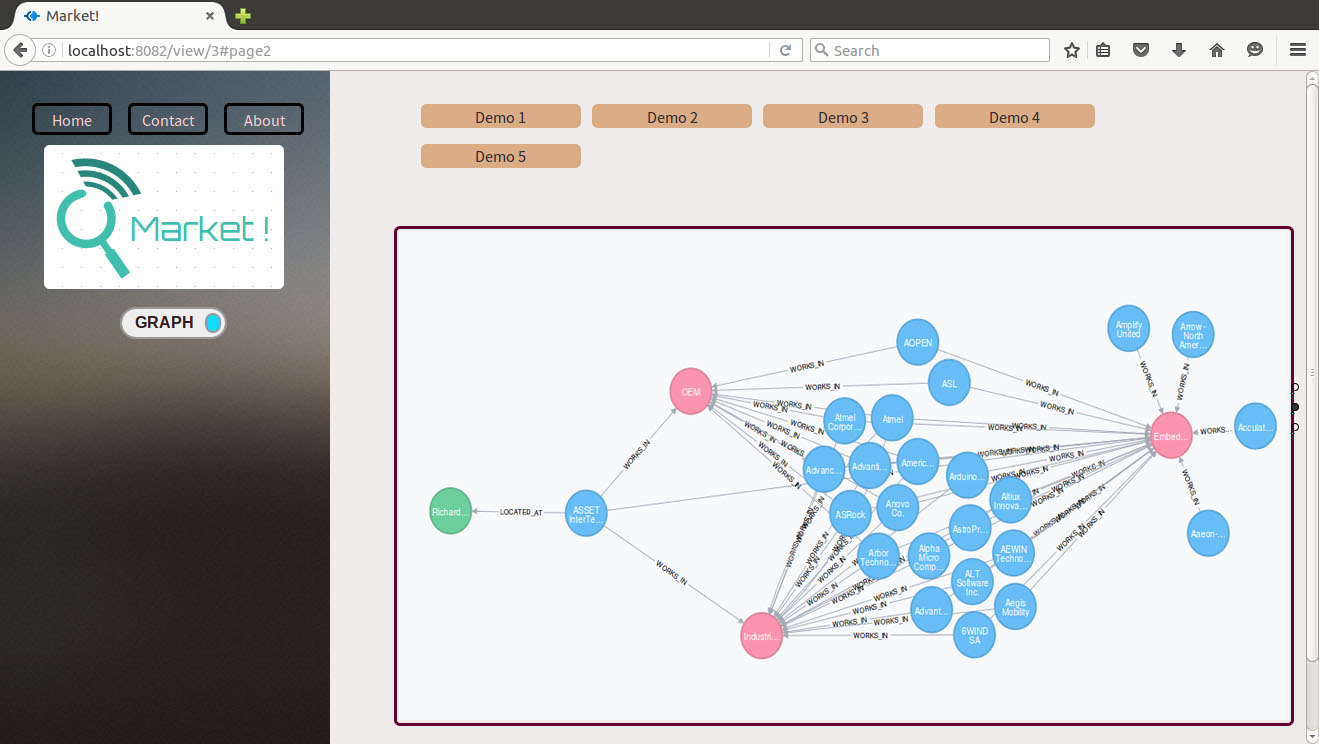
\includegraphics[width=13cm, height=8cm]{d3visual2}
	\centering
	\caption{Example Query: Expanding Nodes}
	\label{fig:d3visual2}
\end{figure}
Figure \ref{fig:d3visual2} shows the screenshot which displays the nodes of OEM, Industrial technology and Embedded technology when expanded.

\begin{figure}[h]
	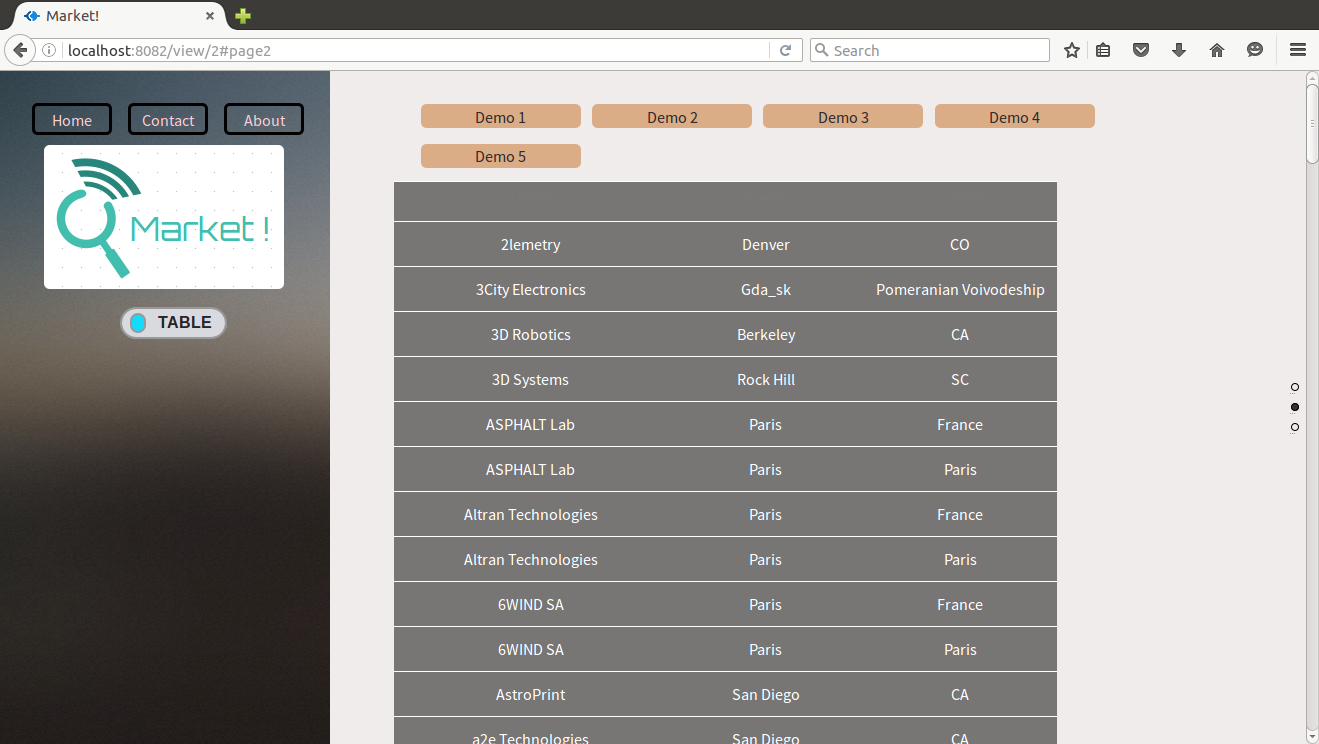
\includegraphics[width=13cm, height=8cm]{tableview}
	\centering
	\caption{Example Query: Companies Locations}
	\label{fig:tableview}
\end{figure}
Figure \ref{fig:tableview} shows the screenshot which displays table visualization of a query.


\begin{figure}[h]
	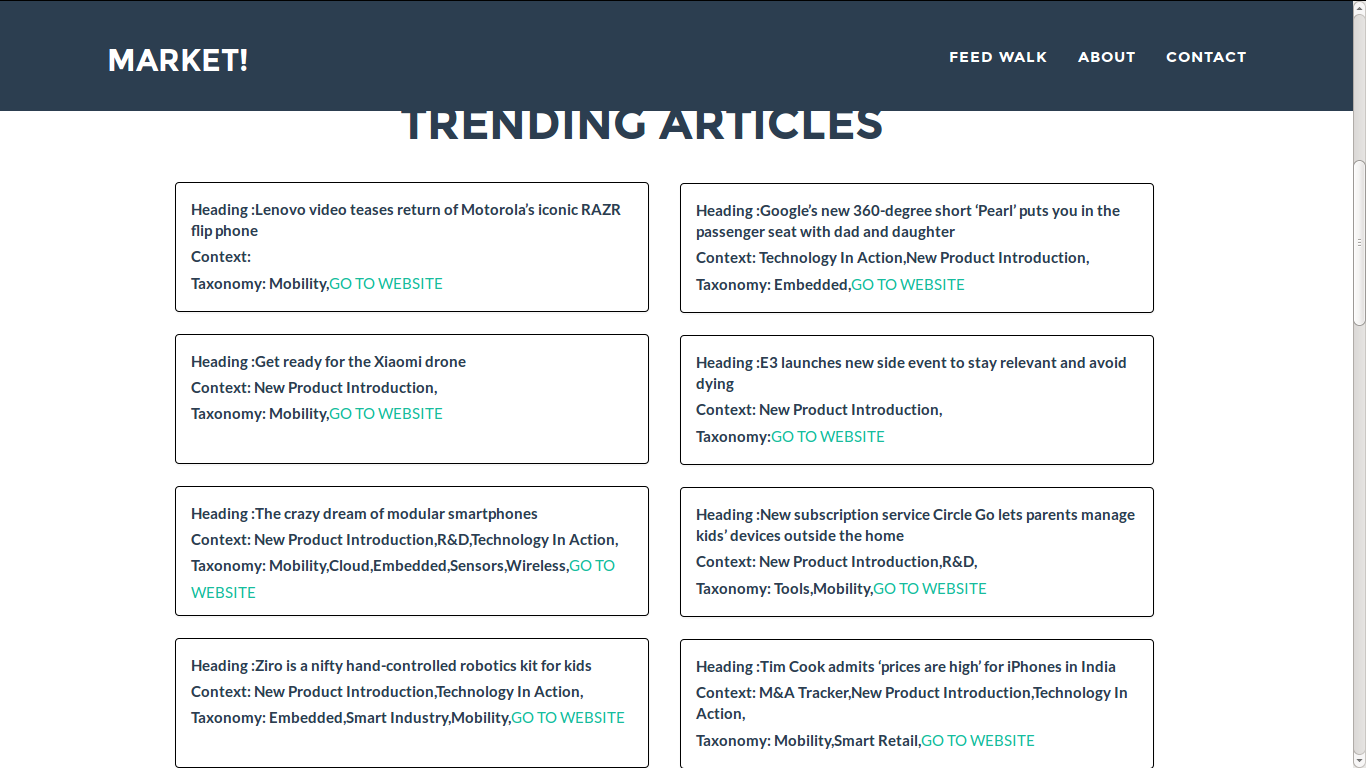
\includegraphics[width=13cm, height=8cm]{newsarticles}
	\centering
	\caption{website diplays latest query information}
	\label{fig:newsarticles}
\end{figure}
Figure \ref{fig:newsarticles} shows the screenshot of the website which provide the latest technology related information.